\lecture{1}{Introduction to Advanced System Architectures}{September 13, 2026}

\subsection{Overview}

This lecture sets up the vocabulary for the rest of the course: what computer
architecture is, how technology trends (Moore's Law, the power wall) pushed the
industry from fast uniprocessors to multicore chips, how the cost of a chip is
determined, and---most importantly---how to \emph{measure and compare
performance} using execution time, the CPU equation, and Amdahl's Law.

\subsection{Course Organization}

\subsubsection{Administrative issues}
\begin{itemize}
  \item \textbf{Textbook:} J.~Hennessy, D.~Patterson, \emph{Computer
  Architecture: A Quantitative Approach}, 5th ed., Morgan Kaufmann, 2012
  (main reference); W.~Stallings, \emph{Computer Organization and
  Architecture}, 7th ed.; K.~Hwang, \emph{Advanced System Architectures:
  Parallelism, Scalability, Programmability}; plus IEEE/ACM research papers.
  \item \textbf{Grades:} 20\% homework + quizzes, 30\% assignments +
  presentations, 50\% final exam.
\end{itemize}

\subsubsection{Course coverage}
\begin{itemize}
  \item \textbf{Introduction} -- brief history of computers, basic concepts
  of computer system architectures.
  \item \textbf{Instruction Set Principles} -- classifying ISAs, addressing
  modes, operand types/sizes, operations, control-flow instructions,
  instruction format, the role of compilers.
  \item \textbf{Pipelining} -- basic and intermediate concepts, organization
  of pipelined units, pipeline hazards, reducing branch penalties, branch
  prediction.
  \item \textbf{Memory Hierarchy Design} -- memory hierarchy, cache
  memories, virtual memories, memory management.
  \item \textbf{Multiprocessors} -- classification and performance of
  parallel architectures, cache coherence.
  \item \textbf{Superscalar \& VLIW} -- superscalar vs.\ superpipelined
  design, instruction dependences, instruction-level parallelism, VLIW.
  \item \textbf{AI \& Security chips.}
\end{itemize}

\subsubsection{Prerequisites}
Computer Organization \& Architecture (combinational/sequential logic,
processor, memory, assembly language); Data Structures/Algorithms
(complexity analysis, efficient implementations); Operating Systems (task
scheduling, management of processors, memory, I/O devices).

% ==========================================================================
\subsection{What is Computer Architecture?}

\subsubsection{A changing definition}
\begin{itemize}
  \item \textbf{1950s--60s:} Computer Arithmetic.
  \item \textbf{1970s--mid-80s:} Instruction Set Design.
  \item \textbf{1990s:} Design of CPU, memory system, I/O system,
  multiprocessors, networks.
  \item \textbf{2000s:} Multi-core design, on-chip networking, parallel
  programming paradigms, power reduction.
  \item \textbf{2010s:} Low-power/mobile processing, self-adapting systems.
  \item \textbf{2020s:} AI chips, quantum computing.
\end{itemize}

\subsubsection{Role of a computer architect}
\begin{definition}[Role of a computer architect]
To design and engineer the various levels of a computer system to
maximize \textbf{performance} and \textbf{programmability} within limits
of \textbf{technology} and \textbf{cost}.
\end{definition}

\subsubsection{The task of the computer designer}
\begin{itemize}
  \item Determine what attributes are important for a new machine.
  \item Design a machine to maximize cost-performance.
  \item What are these tasks?
  \begin{itemize}
    \item Instruction set design
    \item Functional organization
    \item Logic design
    \item Implementation: IC design, packaging, power, cooling, \dots
  \end{itemize}
\end{itemize}

\subsubsection{Levels of abstraction}

Software and hardware consist of hierarchical layers of abstraction, each
hiding the details of the layers below it from the layer above.

\begin{definition}[Instruction Set Architecture]
The \emph{Instruction Set Architecture} (ISA) is the layer that abstracts the
hardware/software interface. It allows many implementations of varying cost
and performance to run the same software.
\end{definition}

\begin{center}
\begin{tikzpicture}[x=1.25cm,y=0.72cm,font=\small\sffamily\bfseries,
  box/.style={draw=black!55,fill=ForestGreen!14,line width=0.5pt}]
  \newcommand{\layer}[5][]{%
    \draw[box,#1] (#2,#3) rectangle (#4,#3+1) node[midway]{#5};}
  % --- software (top to bottom: staircase) ---
  \layer{1.8}{3.15}{8.1}{Application}
  \layer{0}{3}{2.5}{Compiler}
  \layer{0}{2}{2.7}{Assembler}
  \layer{2.7}{2}{10}{Operating System}
  \layer{0}{1}{2.3}{Linker}
  \layer{2.3}{1}{4.5}{Loader}
  \layer{4.5}{1}{7.4}{Scheduler}
  \layer{7.4}{1}{10}{Device Drivers}
  % --- the interface ---
  \draw[box] (-0.9,0) rectangle (10.4,1)
    node[midway,text=ForestGreen!80!black]{Instruction Set Architecture (Interface S/H)};
  % --- hardware ---
  \layer{0}{-1}{3.2}{Processor}
  \layer{3.2}{-1}{6.7}{Memory}
  \layer{6.7}{-1}{10}{I/O System}
  \layer{0}{-2}{10}{Datapath \& Control Design}
  \layer{0}{-3}{10}{Digital Logic Design}
  \layer{0}{-4}{10}{Circuit Design}
  \layer{0}{-5}{10}{Physical (IC Layout) Design}
  % --- side arrows ---
  \draw[-{Latex[length=2.5mm]},thick,ForestGreen!80!black] (-0.45,1.05) -- (-0.45,4.15)
    node[midway,left,rotate=90,anchor=south,text=ForestGreen!80!black]{Software};
  \draw[-{Latex[length=2.5mm]},thick,ForestGreen!80!black] (-0.45,-0.05) -- (-0.45,-5)
    node[midway,left,rotate=90,anchor=south,text=ForestGreen!80!black]{Hardware};
\end{tikzpicture}
\end{center}

% ==========================================================================
\subsection{A Brief History}

\begin{itemize}
  \item \textbf{``Big Iron'' computers} (e.g.\ ENIAC 1945, IBM Mark~1 1944):
  used vacuum tubes, electric relays and bulk magnetic storage devices. No
  microprocessors, no (stored-program) memory.
  \item \textbf{Von Neumann}: invented EDSAC (1949), the first
  \emph{stored-program computer} -- uses memory to hold both instructions
  and data. \emph{We are still using this same basic design today.}
  \item \textbf{The processor chip}: the microprocessor evolution --
  Intel 4004 (1971) $\to$ 8086 (1978) $\to$ 80386 $\to$ 80486 $\to$
  Pentium $\to$ Pentium~II/III $\to \dots \to$ multi-core Core~i7, and
  today's Arrow~Lake / Panther~Lake (2026).
\end{itemize}

\subsubsection{Selected microprocessor milestones (die data)}

\begin{center}
\begin{tabular}{@{}lrrrl@{}}
\toprule
Chip & Year & Transistors & Area & Notes \\
\midrule
Intel 4004      & 1970 & 2,250      & 12 mm$^2$  & first microprocessor, 108 KHz \\
Intel 8086      & 1979 & 29,000     & 33 mm$^2$  & 5 MHz; basis of IA32 PC \\
Intel 80486     & 1989 & 1,200,000  & 81 mm$^2$  & 25 MHz; 1st pipelined IA32 \\
Pentium         & 1993 & 3,100,000  & 296 mm$^2$ & 60 MHz; 1st superscalar IA32 \\
Pentium~III     & 1999 & 9,500,000  & 125 mm$^2$ & 450 MHz \\
\bottomrule
\end{tabular}
\end{center}

\subsubsection{Intel x86 evolution: milestones}

\begin{center}
\begin{tabular}{@{}lrrrp{6cm}@{}}
\toprule
Name & Date & Transistors & MHz & Notes \\
\midrule
8086     & 1978 & 29K   & 5--10     & First 16-bit Intel processor; basis for IBM PC \& DOS; 1MB address space \\
386      & 1985 & 275K  & 16--33    & First 32-bit Intel processor (IA32); flat addressing, can run Unix \\
Pentium 4E & 2004 & 125M & 2800--3800 & First 64-bit Intel x86 processor (x86-64) \\
Core 2   & 2006 & 291M  & 1060--3333 & First multi-core Intel processor \\
Core i7  & 2008 & 731M  & 1600--4400 & Four cores \\
\bottomrule
\end{tabular}
\end{center}

\subsubsection{Process technology}

\begin{center}
\begin{tabular}{@{}lr@{}}
\toprule
Generation & Process node \\
\midrule
1st Pentium Pro (1995) & 600 nm \\
1st Pentium III (1999) & 250 nm \\
1st Pentium 4 (2000)   & 180 nm \\
1st Core 2 Duo (2006)  & 65 nm \\
Nehalem (2008)         & 45 nm \\
Sandy Bridge (2011)    & 32 nm \\
Ivy/Haswell/Broadwell/Skylake/Kaby/Coffee Lake (2012--2017) & 22--14 nm \\
Ice/Tiger/Alder/Raptor Lake (2021--2023) & 10 nm \\
Meteor / Lunar Lake (2024) & 5--7 nm \\
Arrow Lake (2026)      & 3 nm \\
Panther Lake (2026)    & $\sim$2 nm (Intel 18A) \\
\bottomrule
\end{tabular}
\end{center}
Process technology dimension = width of narrowest wires (10 nm $\approx$ 100
atoms wide).

\subsubsection{Moore's Law}
\begin{definition}[Moore's Law]
The number of transistors on a cost-effective integrated circuit doubles
every 18--24 months. (Gordon Moore, ``Cramming More Components onto
Integrated Circuits,'' \emph{Electronics}, 1965.)
\end{definition}
Transistor count has grown from a few thousand (1970s) to over 100 billion
transistors/chip today (e.g.\ Apple M2 Ultra, $\sim$134~billion).

\begin{center}
\begin{tikzpicture}[font=\scriptsize]
  \draw[->] (0,0) -- (10.2,0) node[below]{Year};
  \draw[->] (0,0) -- (0,5.5);
  \node[rotate=90] at (-1.1,2.75) {Transistor count (log scale)};
  \foreach \x/\lab in {0/1970,2.25/1980,4.5/1990,6.75/2000,9/2010}
    \node[below] at (\x,0) {\lab};
  \foreach \y/\lab in {0.5/$10^3$,1.5/$10^4$,2.5/$10^5$,3.5/$10^6$,4.5/$10^7$}
    \node[left] at (0,\y) {\lab};
  \draw[thick,blue] (0.3,0.5) .. controls (3,1.2) and (5,2.8) .. (9,5.2);
  \node[blue,anchor=west] at (5.2,3.6) {doubling every $\sim$2 years};
\end{tikzpicture}
\end{center}
\begin{remark}
The plot above is a schematic reconstruction of the trend, not the original
dataset from the slides.
\end{remark}

\subsubsection{The end of the uniprocessor era}

\begin{itemize}
  \item ``\dots today's processors \dots are nearing an impasse as
  technologies approach the speed of light\dots'' -- David Mitchell, \emph{The
  Transputer: The Time Is Now} (1989).
  \item Custom multiprocessors strove to lead uniprocessors
  $\Rightarrow$ procrastination rewarded: 2$\times$ sequential
  performance / 1.5~years (historically).
  \item ``We are dedicating all of our future product development to
  multicore designs \dots This is a sea change in computing'' -- Paul
  Otellini, President, Intel (2004).
  \item All major microprocessor makers (AMD, Intel, IBM, Sun, Apple)
  switched to multicore $\Rightarrow$ procrastination \emph{penalized}: 2$\times$
  sequential performance / 5(?)~years. Biggest programming challenge: going
  from 1 to 2 CPUs.
\end{itemize}

\textbf{Crossroads -- uniprocessor performance growth (from Hennessy \&
Patterson):}
\begin{center}
\begin{tabular}{@{}ll@{}}
\toprule
Era & Annual growth \\
\midrule
VAX (1978--1986)       & $\sim$25\%/year \\
RISC + x86 (1986--2002) & $\sim$52\%/year \\
RISC + x86 (2002--present) & much slower (single-digit \%/year) \\
\bottomrule
\end{tabular}
\end{center}

\subsubsection{Limiting force: power density}
Chip power density has grown from the level of a \emph{hot plate}
(1980s), past a \emph{nuclear reactor} (1990s), toward a \emph{rocket
nozzle} and approaching the \emph{Sun's surface} by extrapolation --
motivating a shift away from simply raising clock frequency.

\begin{center}
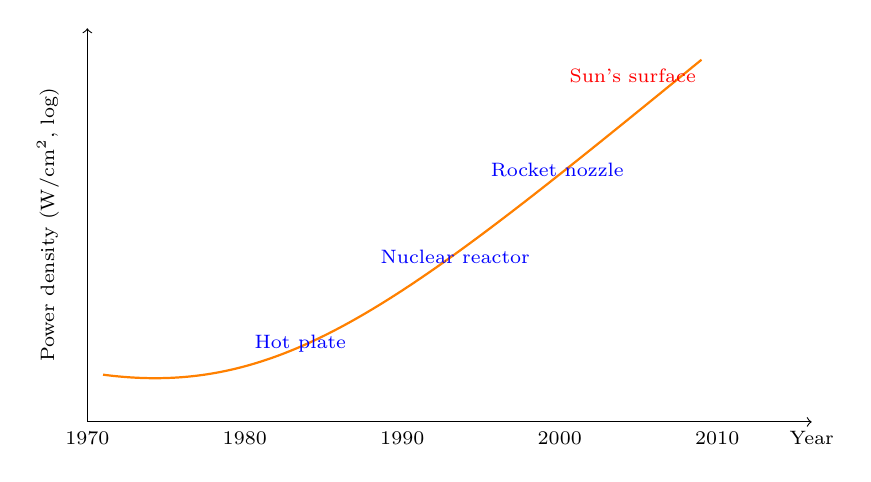
\begin{tikzpicture}[font=\scriptsize]
  \draw[->] (0,0) -- (9.2,0) node[below]{Year};
  \draw[->] (0,0) -- (0,5);
  \node[rotate=90] at (-0.5,2.5) {Power density (W/cm$^2$, log)};
  \foreach \x/\lab in {0/1970,2/1980,4/1990,6/2000,8/2010}
    \node[below] at (\x,0) {\lab};
  \draw[thick,orange] (0.2,0.6) .. controls (2.5,0.3) and (4,1.5) .. (7.8,4.6);
  \node[anchor=west,red] at (6.0,4.4) {Sun's surface};
  \node[anchor=west,blue] at (5.0,3.2) {Rocket nozzle};
  \node[anchor=west,blue] at (3.6,2.1) {Nuclear reactor};
  \node[anchor=west,blue] at (2.0,1.0) {Hot plate};
\end{tikzpicture}
\end{center}

\subsubsection{Conventional wisdom, revisited}
\begin{center}
\begin{tabular}{@{}p{6.6cm}p{6.6cm}@{}}
\toprule
Old conventional wisdom & New conventional wisdom \\
\midrule
Power is free, transistors expensive &
\textbf{``Power wall''}: power expensive, transistors free (can put more on
a chip than can afford to turn on) \\
Increase ILP via compilers, out-of-order, speculation, VLIW &
\textbf{``ILP wall''}: law of diminishing returns on more hardware for ILP \\
Multiplies are slow, memory access is fast &
\textbf{``Memory wall''}: memory slow, multiplies fast ($\sim$200 clock
cycles to DRAM vs.\ 4 clocks for a multiply) \\
Uniprocessor performance $2\times$/1.5~yrs &
Power Wall + ILP Wall + Memory Wall = \textbf{Brick Wall}: uniprocessor
performance now $2\times$/5(?)~yrs \\
\bottomrule
\end{tabular}
\end{center}
\begin{note}
Power Wall + ILP Wall + Memory Wall $\Rightarrow$ a sea change in chip
design: multiple ``cores'' (roughly $2\times$ processors/chip every $\sim$2
years). It is more power-efficient to use many simpler processors than a few
complex ones.
\end{note}

\subsubsection{Sea change in chip design -- an illustration}
\begin{itemize}
  \item Intel 4004 (1971): 4-bit, 2312 transistors, 0.4~MHz, 10~$\mu$m PMOS,
  11~mm$^2$.
  \item RISC~II (1983): 32-bit, 5-stage pipeline, 40{,}760 transistors,
  3~MHz, 3~$\mu$m NMOS, 60~mm$^2$.
  \item A 125~mm$^2$, 65~nm CMOS chip could hold roughly
  $2312\times$(RISC~II + FPU + Icache + Dcache) -- \emph{``the processor is
  the new transistor.''}
\end{itemize}

\subsubsection{ManyCore chips}
\begin{itemize}
  \item Intel 80-core research chip (Feb 2007): 80 simple cores, two
  FP-engines/core, mesh network, 100M transistors, 65 nm.
  \item Intel Single-Chip Cloud Computer (Aug 2010): 24 ``tiles'' with two
  IA cores/tile, 24-router mesh network (256 GB/s bisection bandwidth), 4
  integrated DDR3 controllers, HW support for message-passing.
  \item Open questions: how to program dozens/hundreds of cores? (e.g.\
  dedicate cores to video/audio, one to the browser, dozens to virus
  scanning?) -- something fundamentally new is needed in the
  software/architecture stack.
\end{itemize}

% ==========================================================================
\subsection{The Computer Design Cycle}

A recurring three-part cycle drives computer design:

\begin{enumerate}
  \item \textbf{Performance}: evaluate existing systems for bottlenecks
  using \emph{benchmarks}.
  \item \textbf{Technology}: simulate new designs and organizations, guided
  by \emph{workloads} and \emph{technology trends}.
  \item \textbf{Cost}: implement the next-generation system, weighing
  \emph{implementation complexity} against cost.
\end{enumerate}

\begin{center}
\begin{tikzpicture}[font=\scriptsize,>=Stealth]
  \draw[very thick,red,-{Stealth[length=4mm]}] (90:2) arc (90:-30:2);
  \draw[very thick,green!50!black,-{Stealth[length=4mm]}] (-30:2) arc (-30:-150:2);
  \draw[very thick,blue,-{Stealth[length=4mm]}] (-150:2) arc (-150:-270:2);
  \node[align=center] at (40:2.7) {\textbf{1: Performance}\\Evaluate Existing Systems\\for Bottlenecks\\\emph{using Benchmarks}};
  \node[align=center] at (-90:2.9) {\textbf{2: Technology}\\Simulate New Designs\\and Organizations\\\emph{using Workloads}};
  \node[align=center] at (200:2.7) {\textbf{3: Cost}\\Implement Next\\Generation System\\\emph{Implementation Complexity}};
  \node[align=center] at (0,0) {\textbf{Performance,}\\\textbf{Technology,}\\\textbf{and Cost}};
\end{tikzpicture}
\end{center}

% ==========================================================================
\subsection{Performance and Cost}

\subsubsection{Performance metrics}
\begin{definition}[Latency and throughput]
\textbf{Time / latency} is the wall-clock or CPU elapsed time of a task.
\textbf{Throughput} is the number of results produced per second.
\end{definition}
\begin{remark}
Other measures (MIPS, MFLOPS, clock frequency, cache size) \emph{do not make
sense} on their own as performance measures.
\end{remark}

\subsubsection{Measuring tools}
Benchmarks; hardware cost/delay/area/power consumption; simulation (at ISA,
RT, gate, or circuit levels); queuing theory; fundamental laws/principles.

\subsubsection{Price vs.\ cost}
\begin{definition}[Cost and price]
The \textbf{cost} is the total amount spent to produce a product. The
\textbf{price} is the amount for which a finished good is sold.
\end{definition}
The cost passes through several stages before becoming price; a small
change in cost can have a large impact on price.

\paragraph{Manufacturing cost breakdown.}
\begin{itemize}
  \item \textbf{Component cost}: cost at which components (CPU, DRAM, disk,
  case, \dots) are available to the designer -- typically 40--50\% of list
  price.
  \item \textbf{Direct cost} (recurring): labor, purchasing, scrap,
  warranty -- typically 4--16\% of list price.
  \item \textbf{Gross margin} (non-recurring): R\&D, marketing, sales,
  equipment, rental, maintenance, financing, pre-tax profit, taxes.
  \item \textbf{Average discount}: volume discounts and/or retailer markup,
  typically 15--35\% of list price.
\end{itemize}

\begin{center}
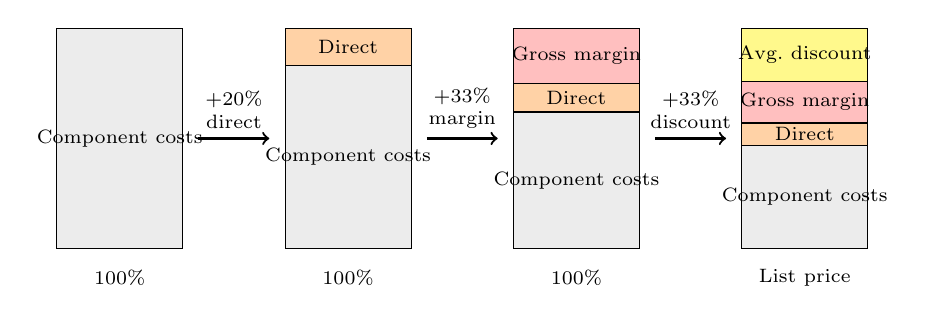
\begin{tikzpicture}[font=\scriptsize,y=0.028cm]
  \def\barw{1.6}
  % stage 1: component costs only, 100%
  \draw[fill=gray!15] (0,0) rectangle ++(\barw,100) node[midway]{Component costs};
  \node[below] at (\barw/2,-5) {100\%};
  \draw[->,thick] (\barw+0.2,50) -- ++(0.9,0) node[midway,above,align=center]{\scriptsize +20\%\\\scriptsize direct};
  % stage 2: + direct costs (17%), component 83%
  \draw[fill=gray!15] (\barw+1.3,0) rectangle ++(\barw,83) node[midway]{Component costs};
  \draw[fill=orange!35] (\barw+1.3,83) rectangle ++(\barw,17) node[midway]{Direct};
  \node[below] at (\barw+1.3+\barw/2,-5) {100\%};
  \draw[->,thick] (2*\barw+1.5,50) -- ++(0.9,0) node[midway,above,align=center]{\scriptsize +33\%\\\scriptsize margin};
  % stage 3: + gross margin, component 62%, direct 13%, margin 25%
  \draw[fill=gray!15] (2*\barw+2.6,0) rectangle ++(\barw,62) node[midway]{\scriptsize Component costs};
  \draw[fill=orange!35] (2*\barw+2.6,62) rectangle ++(\barw,13) node[midway]{\scriptsize Direct};
  \draw[fill=red!25] (2*\barw+2.6,75) rectangle ++(\barw,25) node[midway]{\scriptsize Gross margin};
  \node[below] at (2*\barw+2.6+\barw/2,-5) {100\%};
  \draw[->,thick] (3*\barw+2.8,50) -- ++(0.9,0) node[midway,above,align=center]{\scriptsize +33\%\\\scriptsize discount};
  % stage 4: + avg discount, component 47%, direct 10%, margin 19%, discount 25%
  \draw[fill=gray!15] (3*\barw+3.9,0) rectangle ++(\barw,47) node[midway]{\scriptsize Component costs};
  \draw[fill=orange!35] (3*\barw+3.9,47) rectangle ++(\barw,10) node[midway]{\scriptsize Direct};
  \draw[fill=red!25] (3*\barw+3.9,57) rectangle ++(\barw,19) node[midway]{\scriptsize Gross margin};
  \draw[fill=yellow!45] (3*\barw+3.9,76) rectangle ++(\barw,24) node[midway]{\scriptsize Avg.\ discount};
  \node[below] at (3*\barw+3.9+\barw/2,-5) {List price};
\end{tikzpicture}
\end{center}

\begin{center}
\begin{tabular}{@{}lccc@{}}
\toprule
Component (\% of list price) & Mini & W/S & PC \\
\midrule
Component costs & $\sim$20\% & $\sim$27\% & $\sim$55\% \\
Direct costs     & $\sim$8\%  & $\sim$8\%  & $\sim$5\%  \\
Gross margin     & $\sim$47\% & $\sim$32\% & $\sim$20\% \\
Average discount & $\sim$25\% & $\sim$33\% & $\sim$20\% \\
\bottomrule
\end{tabular}
\end{center}
List price includes an average discount of 15--35\% (volume discounts
and/or retailer markup).

\subsubsection{Cost-effective IC design}
\begin{definition}[Yield, volume, feature size]
\textbf{Yield} is the percentage of manufactured components surviving
testing. \textbf{Volume} is the number of units manufactured; higher volume
decreases the list price and improves purchasing efficiency. \textbf{Feature
size} is the minimum size of a transistor or wire in either $x$ or $y$.
\end{definition}
Reduction in feature size from 10~$\mu$m (1971) to 0.045~$\mu$m (2008) has
produced a quadratic rise in transistor count, a linear increase in
performance, and a jump from 4-bit to 64-bit microprocessors.

\subsubsection{Cost of integrated circuits}
Manufacturing stages: wafer growth and testing $\to$ chopping the wafer into
\emph{dies} $\to$ packaging dies into \emph{chips} $\to$ testing a chip. Dies
near the round wafer periphery are wasted (``waist'' area) since only whole
squares fit.

\begin{center}
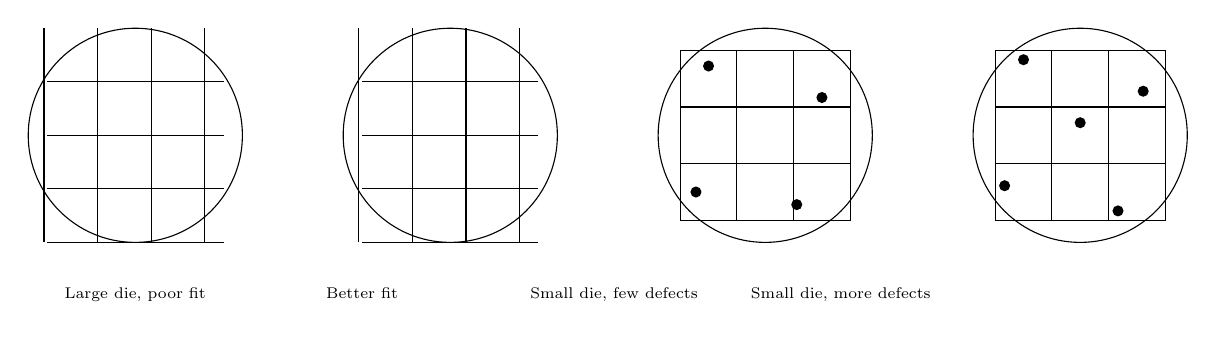
\begin{tikzpicture}[font=\scriptsize,scale=0.8,every node/.style={scale=0.8}]
  \foreach \ox/\lab in {0/{Large die, poor fit},3.6/{Better fit},7.6/{Small die, few defects},11.2/{Small die, more defects}}
    \node[below] at (\ox+1.4,-2.3) {\lab};
  % wafer 1: 4x4 grid, poor fit
  \draw (1.4,0) circle (1.7);
  \foreach \i in {0,...,3} \draw (0,\i*0.85-1.7) -- (2.8,\i*0.85-1.7);
  \foreach \i in {0,...,3} \draw (\i*0.85-0.05,-1.7) -- (\i*0.85-0.05,1.7);
  % wafer 2
  \begin{scope}[xshift=5cm]
  \draw (1.4,0) circle (1.7);
  \foreach \i in {0,...,3} \draw (0,\i*0.85-1.7) -- (2.8,\i*0.85-1.7);
  \foreach \i in {0,...,3} \draw (\i*0.85-0.05,-1.7) -- (\i*0.85-0.05,1.7);
  \end{scope}
  % wafer 3: small die grid with defect dots
  \begin{scope}[xshift=10cm]
  \draw (1.4,0) circle (1.7);
  \foreach \i in {-1,...,1} \foreach \j in {-1,...,1}
    \draw (\i*0.9-0.45+1.4,\j*0.9-0.45) rectangle ++(0.9,0.9);
  \foreach \p in {(0.5,1.1),(2.3,0.6),(0.3,-0.9),(1.9,-1.1)}
    \fill \p circle (2.5pt);
  \end{scope}
  % wafer 4
  \begin{scope}[xshift=15cm]
  \draw (1.4,0) circle (1.7);
  \foreach \i in {-1,...,1} \foreach \j in {-1,...,1}
    \draw (\i*0.9-0.45+1.4,\j*0.9-0.45) rectangle ++(0.9,0.9);
  \foreach \p in {(0.5,1.2),(2.4,0.7),(0.2,-0.8),(2.0,-1.2),(1.4,0.2)}
    \fill \p circle (2.5pt);
  \end{scope}
\end{tikzpicture}
\end{center}

\begin{definition}[Die]
A \emph{die} is the square area of the wafer containing the integrated
circuit. Its cost is determined by the cost of a wafer, the number of dies
that fit on the wafer, and the fraction of dies that work (the
\emph{yield}).
\end{definition}

\begin{prop}[Cost of an integrated circuit]
\begin{align*}
  \text{Cost of IC} &= \frac{\text{die cost} + \text{die testing cost} +
  \text{packaging cost} + \text{final testing cost}}{\text{final test yield}} \\[4pt]
  \text{Die cost} &= \frac{\text{Cost of wafer}}{\text{dies per wafer} \times
  \text{die yield}} \\[4pt]
  \text{Dies per wafer} &= \frac{\pi\,(\text{wafer diameter}/2)^2}{\text{die
  area}} - \frac{\pi\,(\text{wafer diameter})}{\sqrt{2 \times \text{die
  area}}}
\end{align*}
\end{prop}

\begin{eg}[Dies per wafer]
For a die of 0.7~cm on a side, find the number of dies per wafer of 30~cm
diameter:
\[
  \frac{\pi (30/2)^2}{0.49} - \frac{\pi (30)}{\sqrt{2\times 0.49}} = 1347
  \text{ dies}
\]
\end{eg}

\subsubsection{Calculating die yield}
\begin{prop}[Die yield]
Die yield is the fraction of good dies on a wafer. It depends on defect
density $D$ (defects per unit area) and a process-complexity parameter
$\alpha$ (number of masking levels); a good estimate for CMOS is $\alpha
=4.0$:
\[
  \text{Die Yield} = \text{Wafer Yield} \times \left(1 +
  \frac{(\text{Defects/Unit Area}) \times \text{Die Area}}{\alpha}
  \right)^{-\alpha}
\]
\end{prop}

\begin{eg}[Die yield]
The yield of a die 0.7~cm on a side, with defect density 0.6/cm$^2$:
\[
  \left(1 + \frac{0.6 \times 0.49}{4.0}\right)^{-4} = 0.75
\]
\end{eg}

\subsubsection{Real-world example (1993 chip costs)}
\begin{center}
\footnotesize
\begin{tabular}{@{}lrrrrrrrr@{}}
\toprule
Chip & Layers & $\mu$m & Wafer \$ & Def/cm$^2$ &
mm$^2$ & Dies/wf & Yield & Die \$ \\
\midrule
386DX      & 2 & 0.90 & \$900  & 1.0 & 43  & 360 & 71\% & \$4 \\
486DX2     & 3 & 0.80 & \$1200 & 1.0 & 81  & 181 & 54\% & \$12 \\
PowerPC 601& 4 & 0.80 & \$1700 & 1.3 & 121 & 115 & 28\% & \$53 \\
HP PA 7100 & 3 & 0.80 & \$1300 & 1.0 & 196 & 66  & 27\% & \$73 \\
DEC Alpha  & 3 & 0.70 & \$1500 & 1.2 & 234 & 53  & 19\% & \$149 \\
Super SPARC& 3 & 0.70 & \$1700 & 1.6 & 256 & 48  & 13\% & \$272 \\
Pentium    & 3 & 0.80 & \$1500 & 1.5 & 296 & 40  & 9\%  & \$417 \\
\bottomrule
\end{tabular}
\end{center}
\emph{From ``Estimating IC Manufacturing Costs,'' Linley Gwennap,
Microprocessor Report, Aug.\ 2, 1993.}

\subsubsection{Other costs}
\[
  \text{Die Test Cost} = \frac{\text{Test Cost} \times \text{Average Test
  Time}}{\text{Die Yield}}
\]
Packaging cost depends on pin count, heat dissipation, appearance, etc.
Combining die cost with test-and-assembly and packaging gives the total
chip cost -- e.g.\ Pentium (1993): \$417 (die) + \$56 (package + test) =
\$473 total.

\subsubsection{Volume vs.\ cost}
\begin{note}
Rule of thumb (learning-curve effect): ``When volume doubles, costs reduce
10\%.''\; (\emph{A DEC View of Computer Engineering}, C.~G.~Bell,
J.~C.~Mudge, J.~E.~McNamara, 1978.)
\end{note}

\begin{eg}[PC vs.\ workstation volume]
Comparing PC vs.\ workstation shipment volumes (1990--1997), the PC/WS
volume ratio grew from $\sim$59 to $\sim$67 ($2^x = 65 \Rightarrow x
\approx 6.0$), so PC costs fall to roughly $(0.9)^{6.0} = 0.53$ of the
original -- PC costs end up about 47\% lower than workstation costs for the
same functionality.
\end{eg}

\subsubsection{High margins on high-end machines}
R\&D targets a 10\% return on investment: every \$1 of R\&D must generate
\$7--\$13 in sales. High-end machines need more R\&D dollars but sell in
much lower volumes, so they carry much higher margins.

% ==========================================================================
\subsection{Metrics of Performance}

\begin{center}
\begin{tikzpicture}[font=\small,>=Stealth]
  \node[draw,trapezium,trapezium angle=70,minimum height=2cm,minimum width=3.2cm,align=center]
    (t1) at (0,0) {Application\\Programming Language\\Compiler};
  \draw[->] (t1.east) -- ++(1.6,0) node[right,align=left]{Answers per month\\Operations per second};
  \draw[->] ($(t1.south east)+(0,0.3)$) -- ++(1.6,0) node[right,red,align=left]{\textbf{MIPS}: millions of instructions/sec\\\textbf{MFLOPS}: millions of FP ops/sec};
  \node[draw,minimum width=5.4cm,minimum height=0.6cm] (isa) at (0,-1.4) {Instruction Set Architecture};
  \node[draw,trapezium,trapezium angle=-70,minimum height=2cm,minimum width=3.2cm,align=center]
    (t2) at (0,-3.6) {Datapath, Control,\\Function Units,\\Transistors, Pins/Wire--I/O};
  \draw[->] (t2.east) -- ++(1.6,0) node[right,align=left]{Megabytes per second\\Cycles per second (clock rate)};
\end{tikzpicture}
\end{center}

\subsubsection{Time}
\begin{definition}[CPU time]
\textbf{CPU time} is the time the CPU is computing, not including time
waiting for I/O or running other programs. \textbf{User CPU time} is the CPU
time spent in the program; \textbf{system CPU time} is the CPU time spent in
the OS performing tasks requested by the program.
\[ \text{CPU time} = \text{User CPU time} + \text{System CPU time} \]
\end{definition}

\begin{eg}[Unix \texttt{time} command]
\texttt{90.7u 12.9s 2:39 65\%} $\Rightarrow$ user CPU 90.7~s, system CPU
12.9~s, elapsed (response) time $2$:$39 = 159$~s; $(90.7+12.9)/159 \times
100 = 65\%$ of elapsed time is CPU time -- the other 35\% is spent in I/O or
running other programs.
\end{eg}

\subsubsection{Two notions of ``performance''}
\begin{eg}[Boeing 747 vs.\ Concorde]
\leavevmode
\begin{center}
\begin{tabular}{@{}lccccc@{}}
\toprule
Plane & DC to Paris & Speed & Passengers & Throughput (pmph) \\
\midrule
Boeing 747      & 6.5 hours & 610 mph  & 470 & 286,700 \\
BAD/Sud Concorde & 3 hours  & 1350 mph & 132 & 178,200 \\
\bottomrule
\end{tabular}
\end{center}
\begin{itemize}
  \item \textbf{Time to do the task} (execution time, response time,
  latency): Concorde is $1350/610 = 2.2\times$ faster ($=6.5/3$ hours).
  \item \textbf{Tasks per unit time} (throughput, bandwidth): Boeing is
  $286{,}700/178{,}200 = 1.6\times$ ($60\%$) higher throughput; Concorde is
  only $0.62\times$ the Boeing's throughput.
\end{itemize}
\end{eg}
\begin{remark}
Response time and throughput often trade off against each other.
\end{remark}

\subsubsection{Price-performance design: train vs.\ plane}
\begin{eg}[Train vs.\ plane]
\leavevmode
\begin{center}
\begin{tabular}{@{}lccccc@{}}
\toprule
Vehicle & Time lab-to-lab & Passengers/trip & Time to complete job &
Exec.\ time/person \\
\midrule
Train & 4.0 hours & 2400 & 4.0 hours    & 6.0 sec \\
Plane & 45 min    & 300  & 45$\times$8=6.0 hr & 9.0 sec \\
\bottomrule
\end{tabular}
\end{center}
The plane is over $5\times$ faster individually but needs 50\% more time to
finish the whole job (2400 passengers) -- i.e.\ lower throughput; the
train's per-person time and cost are both lower, so its \emph{cost-performance}
is about 15$\times$ better than the plane's (illustrative example).
\end{eg}

% ==========================================================================
\subsection{Comparing Performance and Speedup}

\subsubsection{Execution-time-based performance}
\begin{definition}[Performance and speedup]
For a given program,
\[
  \text{Performance}_A = \frac{1}{\text{Execution Time}_A}.
\]
``Machine A is $n$ times faster than machine B'' (running the same program)
means
\[
  \text{Speedup} = n = \frac{\text{Performance}_A}{\text{Performance}_B} =
  \frac{\text{Execution Time}_B}{\text{Execution Time}_A}.
\]
\end{definition}
\begin{eg}
$\text{Exec}_A = 1$~s, $\text{Exec}_B = 10$~s $\Rightarrow$ Speedup $= 10/1 =
10$: machine A is 10 times faster.
\end{eg}

\subsubsection{The CPU equation}
\begin{theorem}[The CPU equation]
Let a program execute an \emph{instruction count} $I$ (instructions/program),
with an average of $\CPI$ \emph{cycles per instruction}, on a CPU with
\emph{clock cycle time} $C = 1/\text{clock rate}$ (seconds/cycle). Then
\[
  \text{CPU time} = \frac{\text{Seconds}}{\text{Program}} =
  \frac{\text{Instructions}}{\text{Program}} \times
  \frac{\text{Cycles}}{\text{Instruction}} \times
  \frac{\text{Seconds}}{\text{Cycle}},
  \qquad\text{i.e.}\qquad T = I \times \CPI \times C .
\]
\end{theorem}

\begin{eg}[CPU time]
$I = 10{,}000{,}000$ instructions, average $\CPI =2.5$, clock rate
$=200$~MHz ($C = 5\times10^{-9}$~s):
\[
  \text{CPU time} = 10{,}000{,}000 \times 2.5 \times 5\times10^{-9} = 0.125
  \text{ seconds}
\]
\end{eg}

\subsubsection{Factors affecting CPU performance}
\begin{center}
\begin{tabular}{@{}lccc@{}}
\toprule
 & Instruction Count $I$ & CPI & Clock Cycle $C$ \\
\midrule
Program                              & X & X &   \\
Compiler                             & X & X &   \\
Instruction Set Architecture (ISA)   & X & X &   \\
Organization (CPU design)            &   & X & X \\
Technology (VLSI)                    &   &   & X \\
\bottomrule
\end{tabular}
\end{center}

\subsubsection{Performance-comparison example: changing compiler and CPU}
\begin{eg}[New compiler and faster CPU]
Baseline: $I=10{,}000{,}000$, CPI$=2.5$, clock rate $=200$~MHz. With a new
compiler ($I'=9{,}500{,}000$, CPI$'=3.0$) and a faster CPU (clock rate
$=300$~MHz):
\[
  \text{Speedup} = \frac{I \times CPI \times C}{I' \times CPI' \times C'}
  = \frac{10{,}000{,}000\times2.5\times5\times10^{-9}}
         {9{,}500{,}000\times3.0\times3.33\times10^{-9}}
  = \frac{0.125}{0.095} = 1.32
\]
i.e.\ 32\% faster after the changes.
\end{eg}

\subsubsection{Instruction types \& CPI}
\begin{prop}[CPI from instruction classes]
For a program with $n$ instruction classes, $C_i$ = count of instructions of
type $i$, $CPI_i$ = cycles per instruction of type $i$:
\[
  \text{CPU clock cycles} = \sum_{i=1}^{n} \left(CPI_i \times C_i\right)
  \qquad I = \sum_i C_i \qquad CPI = \frac{\text{CPU clock cycles}}{I}
\]
\end{prop}

\begin{eg}[Two code sequences]
3 instruction classes with $CPI_A=1$, $CPI_B=2$, $CPI_C=3$. Two code
sequences:
\begin{center}
\begin{tabular}{@{}lccc@{}}
\toprule
Sequence & $C_A$ & $C_B$ & $C_C$ \\
\midrule
1 & 2 & 1 & 2 \\
2 & 4 & 1 & 1 \\
\bottomrule
\end{tabular}
\end{center}
Sequence 1: cycles $=2(1)+1(2)+2(3)=10$, $I=5$, $CPI=10/5=2$.
Sequence 2: cycles $=4(1)+1(2)+1(3)=9$, $I=6$, $CPI=9/6=1.5$.
\end{eg}

\subsubsection{Instruction frequency \& CPI}
\begin{prop}[CPI from instruction frequencies]
Let $F_i = C_i / I$ be the frequency (fraction) of instruction type $i$.
Then
\[
  CPI = \sum_{i=1}^n \left(CPI_i \times F_i\right)
  \qquad \text{\% of exec.\ time on type } i = \frac{CPI_i \times F_i}{CPI}
\]
\end{prop}

\begin{eg}[RISC typical instruction mix]
\leavevmode
\begin{center}
\begin{tabular}{@{}lccc@{}}
\toprule
Op & $F_i$ & $CPI_i$ & $CPI_i \times F_i$ \\
\midrule
ALU    & 50\% & 1 & 0.50 \\
Load   & 20\% & 5 & 1.00 \\
Store  & 10\% & 3 & 0.30 \\
Branch & 20\% & 2 & 0.40 \\
\midrule
Total  & 100\% & \multicolumn{2}{c}{$CPI = 2.20$} \\
\bottomrule
\end{tabular}
\end{center}
\end{eg}

\subsubsection{Performance terminology}
\begin{definition}[``$n\%$ faster'']
``X is $n\%$ faster than Y'' means
\begin{gather*}
  \frac{\text{ExTime}(Y)}{\text{ExTime}(X)} = \frac{\text{Performance}(X)}
  {\text{Performance}(Y)} = 1 + \frac{n}{100},
  \quad\text{i.e.}\\
  n = \frac{100\,(\text{ExTime}(Y) - \text{ExTime}(X))}{\text{ExTime}(X)}.
\end{gather*}
\end{definition}
\begin{eg}
Y takes 15~s, X takes 10~s: $n = 100(15-10)/10 = 50\%$ faster.
\end{eg}

% ==========================================================================
\subsection{Amdahl's Law}

\begin{theorem}[Amdahl's Law]
The performance improvement to be gained from using a faster mode of
execution is limited by the fraction of time the faster mode can actually be
used. If an enhancement $E$ accelerates a fraction $F$ (Fraction$_{enhanced}$)
of a task by a factor $S$ (Speedup$_{enhanced}$), and the remainder of the
task is unaffected, then
\[
  \text{ExTime}_{new} = \text{ExTime}_{old} \times \left[(1-F) +
  \frac{F}{S}\right]
  \qquad
  \text{Speedup}_{overall} = \frac{1}{(1-F) + \dfrac{F}{S}}.
\]
\end{theorem}

\begin{proof}
Normalize $\text{ExTime}_{old}=1=(1-F)+F$. The unaffected part still takes
$1-F$; the affected part now takes $F/S$. So $\text{ExTime}_{new} =
(1-F)+F/S$, and $\text{Speedup} = \text{ExTime}_{old}/\text{ExTime}_{new}$.
\end{proof}

\begin{explanation}
Even an infinitely fast enhancement ($S\to\infty$) gives at most
$\text{Speedup}\to 1/(1-F)$: the part you did not improve becomes the
bottleneck. $F$ must be a fraction of \emph{execution time}, not of
instruction count.
\end{explanation}

\begin{center}
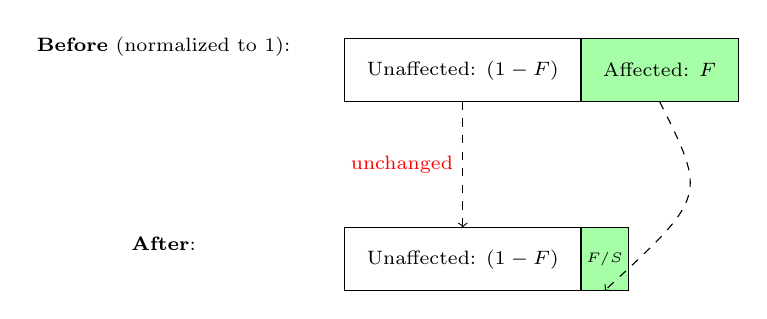
\begin{tikzpicture}[font=\scriptsize]
  \node[align=left] at (-2.3,1.9) {\textbf{Before} (normalized to 1):};
  \draw[fill=white] (0,1.2) rectangle ++(3,0.8) node[midway]{Unaffected: $(1-F)$};
  \draw[fill=green!35] (3,1.2) rectangle ++(2,0.8) node[midway]{Affected: $F$};
  \node[align=left] at (-2.3,-0.6) {\textbf{After}:};
  \draw[fill=white] (0,-1.2) rectangle ++(3,0.8) node[midway]{Unaffected: $(1-F)$};
  \draw[fill=green!35] (3,-1.2) rectangle ++(0.6,0.8) node[midway]{\tiny $F/S$};
  \draw[->,dashed] (1.5,1.2) -- (1.5,-0.4) node[midway,left,red]{unchanged};
  \draw[->,dashed] (4,1.2) .. controls (4.6,0) .. (3.3,-1.2);
\end{tikzpicture}
\end{center}

\subsubsection{Worked examples}

\begin{eg}[Floating point, single enhancement]
FP instructions improved to run $2\times$ faster; only 10\% of instructions
are FP:
\begin{gather*}
  \text{ExTime}_{new} = \text{ExTime}_{old}\times\left((1-0.1) +
  \frac{0.1}{2}\right) = 0.95\,\text{ExTime}_{old}\\
  \text{Speedup} = \frac{1}{0.95} = 1.053
\end{gather*}
\end{eg}

\begin{eg}[RISC load-CPI enhancement]
Using the RISC instruction mix above, a design enhancement improves the CPI of \texttt{Load} from 5 to 2.
\texttt{Load} instructions are 20\% of the instruction count, but the
fraction of \emph{execution time} they affect is what matters for Amdahl's
Law: from the earlier \% Time table, Load accounts for $F=45\% = 0.45$ of
execution time. $S = 5/2 = 2.5$:
\[
  \text{Speedup}(E) = \frac{1}{(1-0.45) + 0.45/2.5} = \frac{1}{0.55+0.18}
  = 1.37
\]
\emph{Cross-check using the CPU equation directly:} Old $CPI = 2.2$; New
$CPI = 0.5(1) + 0.2(2) + 0.1(3) + 0.2(2) = 1.6$;
Speedup $= \text{old }CPI / \text{new }CPI = 2.2/1.6 = 1.37$ -- matches.
\end{eg}

\begin{eg}[How much must multiplication speed up?]
A program runs in 100~s on a machine where multiply operations take 80~s of
that time. By how much must multiply be sped up to make the whole program:
\begin{itemize}
  \item \textbf{4$\times$ faster?} Need ExTime$_{new}=25$s:
  $25 = (100-80) + 80/n \Rightarrow n = 80/5 = 16$; multiply must be
  16$\times$ faster.
  \item \textbf{5$\times$ faster?} Need ExTime$_{new}=20$s:
  $20 = 20 + 80/n \Rightarrow 0 = 80/n$ -- \textbf{impossible}: no amount of
  multiply speed-up can achieve a 5$\times$ overall speedup, since the
  unaffected 20~s alone is already the target time.
\end{itemize}
\end{eg}

\subsubsection{Extending Amdahl's Law to multiple enhancements}
\begin{corollary}[Multiple enhancements]
If enhancements $E_i$ each accelerate a (disjoint) fraction $F_i$ of the
original execution time by factor $S_i$, then
\[
  \text{Speedup} = \frac{1}{\left(1-\sum_i F_i\right) + \sum_i \dfrac{F_i}{S_i}}.
\]
All fractions $F_i$ refer to the \emph{original}, un-enhanced execution time.
\end{corollary}

\begin{eg}[Three enhancements]
$S_1=10, F_1=20\%$; $S_2=15, F_2=15\%$; $S_3=30, F_3=10\%$, each affecting a
disjoint portion of the code, all applied simultaneously:
\begin{align*}
  \text{Speedup} &= \frac{1}{(1-.2-.15-.1) + .2/10 + .15/15 + .1/30}\\
  &= \frac{1}{.55 + .02 + .01 + .0033} = \frac{1}{.5833} = 1.71
\end{align*}
\end{eg}

\subsubsection{Corollary: make the common case fast}
\begin{itemize}
  \item All instructions require an instruction fetch; only a fraction
  require a data fetch/store $\Rightarrow$ optimize instruction access over
  data access.
  \item Programs exhibit \emph{locality} (e.g.\ 90\% of time in 10\% of
  code): spatial locality and temporal locality.
  \item Access to small memories is faster $\Rightarrow$ provide a
  \emph{storage hierarchy} so the most frequent accesses go to the
  smallest, closest memories.
\end{itemize}
\begin{center}
\begin{tikzpicture}[font=\small,>=Stealth]
  \node[draw,minimum width=0.6cm,minimum height=0.6cm] (r) at (0,0) {};
  \node[below] at (0,-0.4) {Reg's};
  \node[draw,minimum width=1.2cm,minimum height=1.2cm] (c) at (1.8,0) {};
  \node[below] at (1.8,-0.8) {Cache};
  \node[draw,minimum width=2cm,minimum height=2cm] (m) at (4.3,0) {};
  \node[below] at (4.3,-1.2) {Memory};
  \node[draw,minimum width=3cm,minimum height=2.6cm] (d) at (8,0) {};
  \node[below] at (8,-1.5) {Disk / Tape};
  \draw[<->] (r) -- (c);
  \draw[<->] (c) -- (m);
  \draw[<->] (m) -- (d);
\end{tikzpicture}
\end{center}

% ==========================================================================
\subsection{Marketing Metrics: MIPS and MFLOPS}

\subsubsection{MIPS}
\begin{definition}[MIPS rating]
\[
  \text{MIPS} = \frac{\text{Instruction Count}}{\text{Execution Time}
  \times 10^6} = \frac{\text{Clock Rate}}{CPI \times 10^6}
\]
\end{definition}
MIPS is a rate of operations per unit time; naive reasoning says a bigger
MIPS rating means a faster machine.

\textbf{Wrong!} Three significant problems with using MIPS:
\begin{enumerate}
  \item \textbf{Instruction-set dependent} -- different machines/ISAs are
  not comparable.
  \item \textbf{Varies between programs} on the \emph{same} computer.
  \item \textbf{Can vary inversely with performance!}
\end{enumerate}

\begin{eg}[Higher MIPS, slower program]
Same machine, instruction classes $A$ (CPI 1), $B$ (CPI 2), $C$ (CPI 3),
clock $=100$~MHz. Two compilers:
\begin{center}
\begin{tabular}{@{}lcccc@{}}
\toprule
Compiler & $C_A$ (M) & $C_B$ (M) & $C_C$ (M) \\
\midrule
1 & 5  & 1 & 1 \\
2 & 10 & 1 & 1 \\
\bottomrule
\end{tabular}
\end{center}
\[
  CPI_1 = \frac{5(1)+1(2)+1(3)}{5+1+1} = \frac{10}{7} = 1.43
  \qquad MIPS_1 = \frac{100}{1.43} = 69.9
\]
\[
  CPI_2 = \frac{10(1)+1(2)+1(3)}{10+1+1} = \frac{15}{12} = 1.25
  \qquad MIPS_2 = \frac{100}{1.25} = 80.0
\]
Compiler~2 has the higher MIPS rating -- so is it faster? Compare CPU
\emph{time} instead:
\[
  \text{CPU time}_1 = \frac{7\times10^6\times1.43}{100\times10^6} = 0.10\text{ s}
  \qquad
  \text{CPU time}_2 = \frac{12\times10^6\times1.25}{100\times10^6} = 0.15\text{ s}
\]
\textbf{Compiler~1's program is actually faster, despite its lower MIPS
rating!} -- because it executes fewer instructions overall.
\end{eg}

\begin{note}
MIPS is valid for comparison only when (1) the same program is used, (2) the
same ISA is used, and (3) the same compiler is used -- i.e.\ the compared
programs are identical down to the instruction count.
\end{note}

\subsubsection{MFLOPS}
\begin{definition}[MFLOPS rating]
\[
  \text{MFLOPS} = \frac{\text{Number of floating-point operations}}
  {\text{Execution time} \times 10^6}
\]
\end{definition}
A floating-point operation is an add/sub/mul/div on single- or
double-precision values. MFLOPS is generally a better cross-machine
comparison than MIPS (applies even across different ISAs), but it is still
\textbf{program-dependent} (different programs have different fractions of
FP ops; a compiler benchmark, with no FP ops, yields MFLOPS $=0$) and
dependent on the \emph{mix} of FP operation types present. A \emph{Peak
MFLOPS} rating -- obtained from a program of only the simplest FP
instructions -- does not represent real FP programs.

% ==========================================================================
\subsection{Benchmarks}

\subsubsection{CPU benchmark suites}
\begin{definition}[Benchmark]
A \emph{benchmark} is a program specifically chosen to measure performance.
\end{definition}
Five levels of programs, in decreasing order of realism/accuracy:
\begin{enumerate}
  \item Real applications
  \item Modified (scripted) applications
  \item Kernels (extracted hot loops)
  \item Toy benchmarks
  \item Synthetic benchmarks
\end{enumerate}

\subsubsection{SPEC (System Performance Evaluation Cooperative)}
\begin{itemize}
  \item \textbf{SPECCPU}: popular desktop CPU-only benchmark suite, split
  into integer and floating-point programs.
  \item \textbf{1989 (1st round)}: 10 programs $\to$ a single SPECmark number.
  \item \textbf{1992 (2nd round)}: SPECint92 (6 integer) and SPECfp92 (14
  FP) programs.
  \item \textbf{1995 (3rd round)}: SPECint95 (8 integer), SPECfp95 (10 FP);
  ``benchmarks useful for 3 years''; a single flag setting for all programs
  (SPECint\_base95, SPECfp\_base95).
  \item \textbf{SPECint2000/SPECfp2000}, and \textbf{SPECCPU2006}.
  \item \textbf{SPECSFS} (NFS file server) and \textbf{SPECWeb} (web
  server) added as server benchmarks.
\end{itemize}

% ==========================================================================
\subsection{Summarizing Performance}

\subsubsection{Arithmetic mean and weighted arithmetic mean}
\[
  \text{Arithmetic mean} = \frac{1}{n}\sum_{i=1}^n T_i \qquad\text{or
  weighted:}\qquad \sum_i W_i \, T_i
\]
Tracks (weighted) \emph{total} execution time, but gives more weight to
longer-running programs, and different weight choices can make different
machines ``look better.''

\begin{eg}[Which machine is better?]
Two programs P1, P2 on three computers:
\begin{center}
\begin{tabular}{@{}lccc@{}}
\toprule
 & Computer A & Computer B & Computer C \\
\midrule
P1 (sec)   & 1    & 10  & 20 \\
P2 (sec)   & 1000 & 100 & 20 \\
Total time & 1001 & 110 & 40 \\
\bottomrule
\end{tabular}
\end{center}
Which machine is ``better''? With three different weighting schemes for
(P1,P2):
\begin{center}
\begin{tabular}{@{}lccc@{}}
\toprule
Weights (P1/P2) & Computer A & Computer B & Computer C \\
\midrule
.5 / .5     & 500.5 & 55.0  & 20 \\
.909 / .091 & 91.82 & 18.8  & 20 \\
.999 / .001 & 2     & 10.09 & 20 \\
\bottomrule
\end{tabular}
\end{center}
Each weighting scheme picks a different ``winner'' -- illustrating why the
choice of weights is itself contentious.
\end{eg}

\subsubsection{Normalized execution time and the geometric mean}
\begin{definition}[Normalized execution time]
Pick a reference machine $R$. The normalized execution time of program $A$
on machine $X$ is (time to run $A$ on $X$) / (time to run $A$ on $R$).
Summarize with the \textbf{geometric mean}
\[
  \sqrt[n]{\prod_{i=1}^{n} \text{Normalized execution time on } i}.
\]
\end{definition}
\begin{remark}
The arithmetic mean of normalized times depends on the choice of reference
machine; the geometric mean is \emph{consistent regardless of the reference
machine}, but it is \emph{not} a good metric for total execution time.
\end{remark}

\subsubsection{Summary of means}
\begin{center}
\begin{tabular}{@{}lcp{4.6cm}@{}}
\toprule
Mean & Formula & Property \\
\midrule
Arithmetic & $\dfrac{1}{n}\sum_i T_i$ & Can be weighted; represents total execution time \\
Harmonic   & $\dfrac{n}{\sum_i 1/R_i}$ & Used for rates (e.g.\ throughput) \\
Geometric  & $\left(\prod_i \dfrac{T_i}{T_{r_i}}\right)^{1/n} =
\exp\!\left(\dfrac{1}{n}\sum_i \log\dfrac{T_i}{T_{r_i}}\right)$ &
Consistent, independent of reference machine \\
\bottomrule
\end{tabular}
\end{center}

\subsubsection{Performance evaluation, in practice}
Sales are, in part, a function of performance relative to the competition,
and companies invest heavily in improving the product as reported by
performance summaries. Good products result from having \emph{good
benchmarks} and \emph{good ways to summarize performance}. If benchmarks or
summaries are inadequate, vendors must choose between improving the product
for real programs vs.\ improving it to score better on the benchmark --
and, cynically, ``sales almost always wins.'' In the end,
\textbf{execution time remains the real measure of computer performance}.

% ==========================================================================
\subsection{Summary}

\begin{itemize}[leftmargin=*]
  \item Chip density continues to increase ($\sim2\times$ every 2 years);
  clock speed has largely stopped scaling, so the number of
  processors/cores per chip increases instead.
  \item Always keep concrete metrics and benchmarks in mind to justify
  comparisons between systems.
  \item \textbf{Amdahl's Law}:
  \[
    \text{Speedup}_{overall} = \frac{\text{ExTime}_{old}}{\text{ExTime}_{new}}
    = \frac{1}{(1-\text{Fraction}_{enhanced}) +
    \dfrac{\text{Fraction}_{enhanced}}{\text{Speedup}_{enhanced}}}
  \]
  \item \textbf{The CPU equation}:
  \[
    \text{CPU time} = \frac{\text{Seconds}}{\text{Program}} =
    \frac{\text{Instructions}}{\text{Program}} \times
    \frac{\text{Cycles}}{\text{Instruction}} \times
    \frac{\text{Seconds}}{\text{Cycle}}
  \]
  \item \textbf{Execution time is the only reliable measure of computer
  performance}; die cost grows roughly with die area to a power greater
  than~1 (quadratically-ish, via the yield model).
  \item ``For better or worse, benchmarks shape a field.'' Good products
  need good benchmarks \emph{and} good ways to summarize performance.
\end{itemize}

